\documentclass{article}

% if you need to pass options to natbib, use, e.g.:
%     \PassOptionsToPackage{numbers, compress}{natbib}
% before loading neurips_2019

% ready for submission
% \usepackage[nonatbib]{neurips_2019_ml4ad}

% to compile a preprint version, e.g., for submission to arXiv, add add the
% [preprint] option:
% \usepackage[preprint, nonatbib]{neurips_2019_ml4ad}

% to compile a camera-ready version, add the [final] option, e.g.:
\usepackage[final, nonatbib]{neurips_2019_ml4ad}

% to avoid loading the natbib package, add option nonatbib:
% \usepackage[nonatbib]{neurips_2019_ml4ad}

\usepackage[utf8]{inputenc} % allow utf-8 input
\usepackage[T1]{fontenc}    % use 8-bit T1 fonts
\usepackage{hyperref}       % hyperlinks
\usepackage{url}            % simple URL typesetting
\usepackage{booktabs}       % professional-quality tables
\usepackage{amsfonts}       % blackboard math symbols
\usepackage{nicefrac}       % compact symbols for 1/2, etc.
\usepackage{microtype}      % microtypography

% Custom packages
\usepackage[round]{natbib}
\usepackage{amsmath}
\usepackage{amssymb}
\usepackage{graphicx}
\usepackage{array, makecell}
\usepackage{tikz}
\usepackage{xspace}
\usepackage{float}
\usetikzlibrary{arrows,automata}
\usepackage{pgfplots}
\usetikzlibrary{intersections}
\usepackage{subcaption}
\usepackage[flushleft]{threeparttable}
\usepackage{cases}
\usepackage{multirow}

\definecolor{mylinkcolor}{HTML}{e83f6f}
\definecolor{mycitecolor}{HTML}{2980B9}
\definecolor{myurlcolor}{HTML}{d63230}
% \definecolor{myalgocolor}{HTML}{32936f}
\definecolor{myalgocolor}{HTML}{000000}
\hypersetup{
	linkcolor  = mylinkcolor,
	citecolor  = mycitecolor,
	urlcolor   = myurlcolor,
	colorlinks = true,
}

\AtBeginDocument{\def\sectionautorefname{Section}}%



%%%%%%%%%%%%%%%%%%%%%%%%%%%%
% Paper dependent stuff    %
%%%%%%%%%%%%%%%%%%%%%%%%%%%%

\newcommand{\MLPL}{\texttt{MLP/List}\xspace}
\newcommand{\MLPG}{\texttt{MLP/Grid}\xspace}
\newcommand{\EgoAtt}{\texttt{Ego-Attention}\xspace}


%%%%%%%%%%%%%%%%%%%%%%%%%%%%
% Aesthetics               %
% over-underline, hat, bold%
%%%%%%%%%%%%%%%%%%%%%%%%%%%%

\newcommand{\eps}{\varepsilon}
\newcommand{\vareps}{\varepsilon}
\renewcommand{\epsilon}{\varepsilon}
%\renewcommand{\hat}{\widehat}
\renewcommand{\tilde}{\widetilde}
\renewcommand{\bar}{\overline}

\newcommand*{\MyDef}{\mathrm{\tiny def}}
\newcommand*{\eqdefU}{\ensuremath{\mathop{\overset{\MyDef}{=}}}}% Unscaled version



\def\:#1{\protect \ifmmode {\mathbf{#1}} \else {\textbf{#1}} \fi}
\newcommand{\CommaBin}{\mathbin{\raisebox{0.5ex}{,}}}

\newcommand{\wt}[1]{\widetilde{#1}}
\newcommand{\wh}[1]{\widehat{#1}}
\newcommand{\wo}[1]{\overline{#1}}
\newcommand{\wb}[1]{\overline{#1}}

% bf and bm missing due to conflict!!
\newcommand{\bsym}[1]{\mathbf{#1}}
\newcommand{\bzero}{\mathbf{0}}
\newcommand{\ba}{\mathbf{a}}
\newcommand{\bb}{\mathbf{b}}
\newcommand{\bc}{\mathbf{c}}
\newcommand{\bd}{\mathbf{d}}
\newcommand{\be}{\mathbf{e}}
\newcommand{\bg}{\mathbf{g}}
\newcommand{\bh}{\mathbf{h}}
\newcommand{\bi}{\mathbf{i}}
\newcommand{\bj}{\mathbf{j}}
\newcommand{\bk}{\mathbf{k}}
\newcommand{\bl}{\mathbf{l}}
\newcommand{\bn}{\mathbf{n}}
\newcommand{\bo}{\mathbf{o}}
\newcommand{\bp}{\mathbf{p}}
\newcommand{\bq}{\mathbf{q}}
\newcommand{\br}{\mathbf{r}}
\newcommand{\bs}{\mathbf{s}}
\newcommand{\bt}{\mathbf{t}}
\newcommand{\bu}{\mathbf{u}}
\newcommand{\bv}{\mathbf{v}}
\newcommand{\bw}{\mathbf{w}}
\newcommand{\bx}{\mathbf{x}}
\newcommand{\by}{\mathbf{y}}
\newcommand{\bz}{\mathbf{z}}

\newcommand{\bA}{\mathbf{A}}
\newcommand{\bB}{\mathbf{B}}
\newcommand{\bC}{\mathbf{C}}
\newcommand{\bD}{\mathbf{D}}
\newcommand{\bE}{\mathbf{E}}
\newcommand{\bF}{\mathbf{F}}
\newcommand{\bG}{\mathbf{G}}
\newcommand{\bH}{\mathbf{H}}
\newcommand{\bI}{\mathbf{I}}
\newcommand{\bJ}{\mathbf{J}}
\newcommand{\bK}{\mathbf{K}}
\newcommand{\bL}{\mathbf{L}}
\newcommand{\bM}{\mathbf{M}}
\newcommand{\bN}{\mathbf{N}}
\newcommand{\bO}{\mathbf{O}}
\newcommand{\bP}{\mathbf{P}}
\newcommand{\bQ}{\mathbf{Q}}
\newcommand{\bR}{\mathbf{R}}
\newcommand{\bS}{\mathbf{S}}
\newcommand{\bT}{\mathbf{T}}
\newcommand{\bU}{\mathbf{U}}
\newcommand{\bV}{\mathbf{V}}
\newcommand{\bW}{\mathbf{W}}
\newcommand{\bX}{\mathbf{X}}
\newcommand{\bY}{\mathbf{Y}}
\newcommand{\bZ}{\mathbf{Z}}

% calligraphic
\newcommand{\cf}{\mathcal{f}}
\newcommand{\cA}{\mathcal{A}}
\newcommand{\cB}{\mathcal{B}}
\newcommand{\cC}{\mathcal{C}}
\newcommand{\cD}{\mathcal{D}}
\newcommand{\cE}{\mathcal{E}}
\newcommand{\cF}{\mathcal{F}}
\newcommand{\cG}{\mathcal{G}}
\newcommand{\cH}{\mathcal{H}}
\newcommand{\cI}{\mathcal{I}}
\newcommand{\cJ}{\mathcal{J}}
\newcommand{\cK}{\mathcal{K}}
\newcommand{\cL}{\mathcal{L}}
\newcommand{\cM}{\mathcal{M}}
\newcommand{\cN}{\mathcal{N}}
\newcommand{\cO}{\mathcal{O}}
\newcommand{\cP}{\mathcal{P}}
\newcommand{\cQ}{\mathcal{Q}}
\newcommand{\cR}{\mathcal{R}}
\newcommand{\cS}{\mathcal{S}}
\newcommand{\cT}{\mathcal{T}}
\newcommand{\cU}{\mathcal{U}}
\newcommand{\cV}{\mathcal{V}}
\newcommand{\cW}{\mathcal{W}}
\newcommand{\cX}{\mathcal{X}}
\newcommand{\cY}{\mathcal{Y}}
\newcommand{\cZ}{\mathcal{Z}}

%%%%%%%%%%%%%%%%%%%%%%%%%%%%
% Math jargon              %
%%%%%%%%%%%%%%%%%%%%%%%%%%%%
\newcommand{\wrt}{w.r.t.\xspace}
\newcommand{\defeq}{\stackrel{\mathclap{\normalfont\mbox{\tiny def}}}{=}}
\newcommand{\maxund}[1]{\max\limits_{#1}}
\newcommand{\supund}[1]{\text{sup}\limits_{#1}}
\newcommand{\minund}[1]{\min\limits_{#1}}
\renewcommand{\epsilon}{\varepsilon}
\newcommand{\bigotime}{\mathcal{O}}


\DeclareMathOperator*{\argmin}{arg\,min} 
\DeclareMathOperator*{\argmax}{arg\,max} 
\DeclareMathOperator*{\cupdot}{\mathbin{\mathaccent\cdot\cup}}
\newcommand{\eqdef}{\buildrel \text{def}\over =}

%%%%%%%%%%%%%%%%%%%%%%%%%%%%
% Matrix operators         %
%%%%%%%%%%%%%%%%%%%%%%%%%%%%
\newcommand{\transpose}{^\mathsf{\scriptscriptstyle T}}
\newcommand{\transp}{\mathsf{\scriptscriptstyle T}}

%%%%%%%%%%%%%%%%%%%%%%%%%%%%
% Statistic operators      %
%%%%%%%%%%%%%%%%%%%%%%%%%%%%
\newcommand{\probability}[1]{\mathbb{P}\left(#1\right)}
\newcommand{\probdist}{Pr}
\DeclareMathOperator*{\expectedvalue}{\mathbb{E}}
\DeclareMathOperator*{\variance}{\text{Var}}
\newcommand{\expectedvalueover}[1]{\expectedvalue\limits_{#1}}
\newcommand{\condbar}{\;\middle|\;}
\newcommand{\gaussdistr}{\mathcal{N}}
\newcommand{\uniformdistr}{\mathcal{U}}
\newcommand{\bernoullidist}{\mathcal{B}}

%%%%%%%%%%%%%%%%%%%%%%%%%%%%
% Algebraic Sets           %
%%%%%%%%%%%%%%%%%%%%%%%%%%%%
\newcommand{\Real}{\mathbb{R}}
\newcommand{\Natural}{\mathbb{N}}
\newcommand{\statespace}{\mathcal{X}}
\newcommand{\funcspace}{\mathcal{F}}
\newcommand{\dynaspace}{\mathcal{T}}


\newtheorem{theorem}{Theorem}
\newtheorem{definition}{Definition}
\newtheorem{lemma}{Lemma}
\newtheorem{proposition}{Proposition}
\newtheorem{remark}{Remark}
\newtheorem{property}{Property}
\newtheorem{assumption}{Assumption}
\newtheorem{conjecture}{Conjecture}

\title{Social Attention for Autonomous Decision-Making in Dense Traffic}

% The \author macro works with any number of authors. There are two commands
% used to separate the names and addresses of multiple authors: \And and \AND.
%
% Using \And between authors leaves it to LaTeX to determine where to break the
% lines. Using \AND forces a line break at that point. So, if LaTeX puts 3 of 4
% authors names on the first line, and the last on the second line, try using
% \AND instead of \And before the third author name.

%Happy Horizontal People Transporter
%From the Sirius Cybernetics Corporation with a Genuine People Personality

\author{%
	Edouard Leurent\thanks{Equal contribution.} \\
	SequeL team, INRIA Lille -- Nord Europe\\
	Renault Group, France\\
	\texttt{edouard.leurent@inria.fr} \\
	\And
	Jean Mercat$^*$ \\
	Laboratoire des signaux et des syst\`emes, Centrale-Sup\'elec\\
	Renault Group, France\\
	\texttt{jean.mercat@renault.com} \\
}

\begin{document}
	
	
	\tikzset{
		state/.style={
			rectangle,
			draw=black, very thick,
			minimum height=2em,
			inner sep=2pt,
			text centered,
		},
		name plot/.style={every path/.style={name path global=#1}}
	}
	
		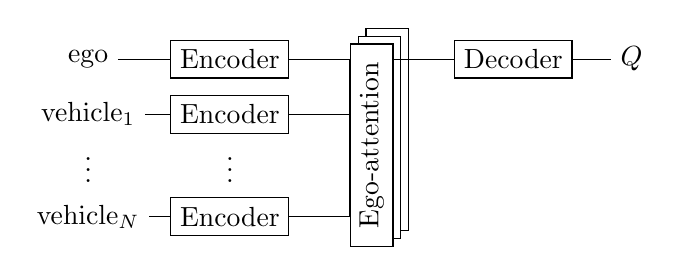
\begin{tikzpicture}
		\node(X1){ego};
		\node[below of=X1, node distance=0.7cm](X2){vehicle$_{1}$};
		\node[below of=X2, node distance=0.6cm](X3){$\vdots$};
		\node[below of=X3, node distance=0.7cm](X4){vehicle$_{N}$};
		
		\node[draw, right of=X1, node distance=1.8cm, rectangle](ENC1){Encoder};
		\node[draw, right of=X2, node distance=1.8cm, rectangle](ENC2){Encoder};
		\node[below of=ENC2, node distance=0.6cm](ENC3){$\vdots$};
		\node[draw, right of=X4, node distance=1.8cm, rectangle](ENC4){Encoder};
		
		\path (X1) edge (ENC1);
		\path (X2) edge (ENC2);
		\path (X4) edge (ENC4);
		
		
		\node[draw, rectangle, right of=ENC1, node distance=2.0cm, below=-0.4cm, fill=white](TRANS3){\rotatebox{90}{ Ego-attention }};
		\node[draw, rectangle, right of=ENC1, node distance=1.9cm, below=-0.3cm, fill=white](TRANS2){\rotatebox{90}{ Ego-attention }};
		\node[draw, rectangle, right of=ENC1, node distance=1.8cm, below=-0.2cm, fill=white](TRANS1){\rotatebox{90}{ Ego-attention }};
		
		\draw (ENC1.east) -| (TRANS1.west);
		\draw (ENC2.east) -| (TRANS1.west);
		\draw (ENC4.east) -| (TRANS1.west);
		
		
		\node[draw, right of=ENC1, node distance=3.6cm, rectangle](DEC1){Decoder};
		
		\draw (TRANS1.east) |- (DEC1.west);
		
		\node[right of=DEC1, node distance=1.5cm](Y1){$Q$};
		
		\draw (DEC1.east) -- (Y1.west);
		\end{tikzpicture}

		\clearpage
		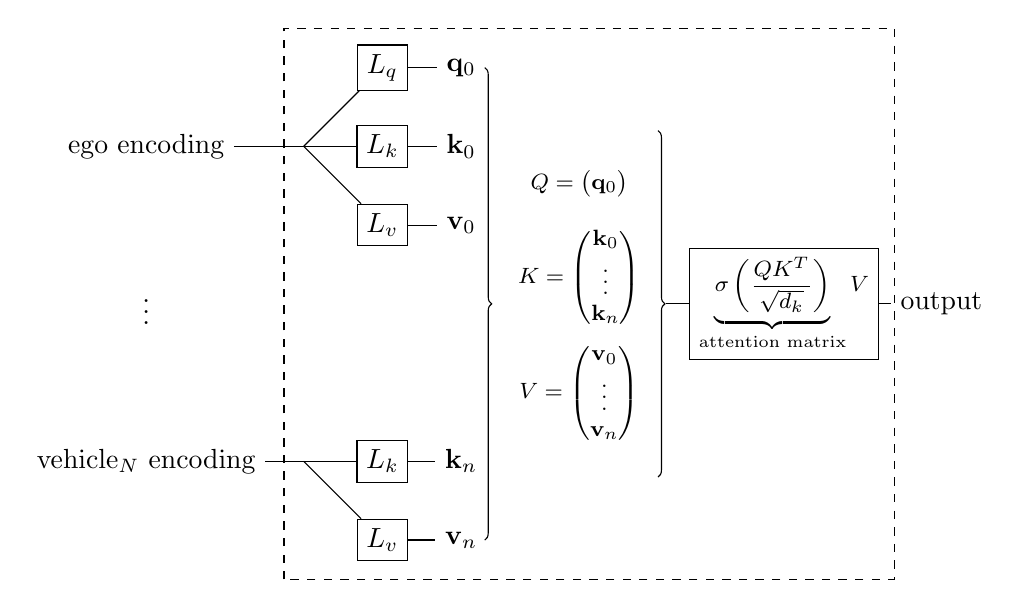
\begin{tikzpicture}[scale=1, every node/.style={scale=1}]
		\node(X1){ego encoding};
		\node[below of=X1, node distance=2cm](X2){$\vdots$};
		\node[below of=X2, node distance=2cm](X3){vehicle$_{N}$ encoding};
		
		\coordinate[right of= X1, node distance=2cm](X1b){};
		
		\draw (X1) -- (X1b);
		
		\node[draw, right of=X1b, node distance=1cm](LK1){$L_{k}$};
		\node[draw, below of=LK1, node distance=1cm](LV1){$L_{v}$};
		\node[draw, above of=LK1, node distance=1cm](LQ1){$L_{q}$};
		
		\draw (X1b) -- (LQ1);
		\draw (X1b) -- (LK1);
		\draw (X1b) -- (LV1);
		
		
		\node[right of=LQ1, node distance=1cm](Q1){$\mathbf{q}_0$};
		\node[right of=LK1, node distance=1cm](K1){$\mathbf{k}_0$};
		\node[right of=LV1, node distance=1cm](V1){$\mathbf{v}_0$};
		
		\draw (LQ1) -- (Q1);
		\draw (LK1) -- (K1);
		\draw (LV1) -- (V1);
		
		\coordinate[right of= X3, node distance=2cm](X3b){};
		
		\draw (X3) -- (X3b);
		
		\node[draw, right of=X3b, node distance=1cm](LK3){$L_{k}$};
		\node[draw, below of=LK3, node distance=1cm](LV3){$L_{v}$};
		
		\draw (X3b) -- (LK3);	
		\draw (X3b) -- (LV3);
		
		\node[right of=LK3, node distance=1cm](K3){$\mathbf{k}_{n}$};
		\node[right of=LV3, node distance=1cm](V3){$\mathbf{v}_{n}$};
		
		\draw (LK3) -- (K3);
		\draw (LV3) -- (V3);
		
		\coordinate[right of=Q1, node distance=0.3cm](TOP){};
		\coordinate[right of=V3, node distance=0.3cm](BOT){};
		\draw[decorate,decoration={brace}] (TOP) -- node[left=5pt]{} (BOT);
		
		\node[right of=X2, text width=3cm, node distance=5.5cm](EQ){
			\footnotesize \[Q = \left( \begin{matrix}
			\mathbf{q}_0
			\end{matrix} \right)\]
			\\
			\footnotesize \[K = \left( \begin{matrix}
			\mathbf{k}_0 \\
			\vdots \\
			\mathbf{k}_{n}
			\end{matrix} \right)\]
			\\
			\footnotesize \[ V = \left( \begin{matrix}
			\mathbf{v}_0 \\
			\vdots \\
			\mathbf{v}_{n}
			\end{matrix}\right) \]
		};
		
		\node[draw, right of=X2, node distance=8.1cm](EQ2){
			\footnotesize $\underbrace{\sigma\left(\frac{QK^T}{\sqrt{d_k}}\right)}_{\text{attention matrix}}V$};
		
		\coordinate[left of=EQ2, node distance=1.6cm, above=2.2cm](TOP2){};
		\coordinate[left of=EQ2, node distance=1.5cm, below=0.0cm](MID2){};
		\coordinate[left of=EQ2, node distance=1.6cm, below=2.2cm](BOT2){};
		\draw[decorate,decoration={brace}] (TOP2) -- node[left=5pt]{} (BOT2);
		\draw (MID2) -- (EQ2);
		
		\node[right of=EQ2, node distance=2cm](OUT){output};
		\draw (EQ2) -- (OUT);
		
		\draw[draw=black, dashed] (1.75cm, -5.5cm) rectangle (9.5cm,1.5cm);
		\end{tikzpicture}


	
	
	
	
\end{document}
